\documentclass{article} % For LaTeX2e
\usepackage{nips13submit_e,times}
\usepackage{hyperref}
\usepackage{url}
\usepackage{graphicx}
\usepackage{epstopdf}
\usepackage{listings}
\lstset{language=Matlab}
\lstset{breaklines}
\lstset{extendedchars=false}
\usepackage{amsmath}
\usepackage{txfonts}
\usepackage{subfigure}
\usepackage{mathrsfs}



\title{Convolutional Neural Network and Convex optimization}


\author{
Si Chen  and   Yufei Wang\\
Department of Electrical and Computer Engineering\\
University of California San Diego\\
\texttt{\{sic046, yuw176\}@ucsd.edu}          \\
}

% The \author macro works with any number of authors. There are two commands
% used to separate the names and addresses of multiple authors: \And and \AND.
%
% Using \And between authors leaves it to \LaTeX{} to determine where to break
% the lines. Using \AND forces a linebreak at that point. So, if \LaTeX{}
% puts 3 of 4 authors names on the first line, and the last on the second
% line, try using \AND instead of \And before the third author name.

\newcommand{\fix}{\marginpar{FIX}}
\newcommand{\new}{\marginpar{NEW}}

\nipsfinalcopy % Uncomment for camera-ready version

\begin{document}


\maketitle
\begin{abstract}
%We model the relationship between sentences and their punctuation labels using conditional random fields. Some feature functions are hand-designed and others are generated by templates. We train the same model by stochastic gradient ascent, Collins Perceptron and contrastive divergence respectively and compare their performance. On the provided dataset, we achieve word-level accuracy of 94.56\%. At last, we propose a heuristic that can deal with cost-sensitive tasks.   
Latent Dirichlet allocation(LDA) is a generative topic model to find latent topics in a text corpus. It can be trained via collapsed Gibbs sampling. In this project, we train LDA models on two datasets, Classic400 and BBCSport dataset. We discuss possible ways to evaluate goodness-of-fit and to detect overfitting problem of LDA model, and we use these criteria to choose proper hyperparameters, observe convergence, and evaluate the models, the criteria we use include perplexity, VI-distance, visualization of clustering results, and highest-probability words. 

\end{abstract}
\section{Introduction}

Deep learning


Convex optimization


SVM-loss



%Latent Dirichlet allocation introduced by \cite{blei} is a generative probabilistic model for collection of discrete data, such as text corpora.It assumes each word is a mixture over an underlying set of topics, and each topic is a mixture over a set of topic probabilities. Evaluating the models is a tough issue. There are several types of methods that people use: The models can be applied to some tasks such as document classification, where the performance can be easily evaluated; Several methods estimate the likelihood of held-out documents; Subjective judgement can be made by examine word and document similarities. In this project, we learn the models of two datasets, Classic400 and BBCSport dataset, by collapsed Gibbs sampling, and use several methods to evaluate the models, including perplexity, VI-distance, visualizing result and highest-probability words.
\par
%This report is organized as follows. Section 2 gives a brief overview of LDA model and training process, and introduces several methods to evaluate goodness-of-fit and check overfitting. We describe some implementation details in Section 3. In Section 4, we describe the design of our experiments. Section 5 shows the experiment results with discussions. Finally, we draw some conclusions in Section 6.

\section{Sub-model Convolutional Network}
\subsection{Theoretical basis: Convolutional neural network}
Convolutional neural networks(CNN) are a special kind of deep neural networks. It exploits local correlation by enforcing a local connectivity pattern between neurons of adjacent layers. For a certain hidden layer $m$, the hidden units in it are connected to a local subset of units in the $(m-1)$th layer. Additionally, each sparse filter $h_{i}$ is replicated across the entire visual field. The replicated units share the same parametrization, i.e. the same weight vector and same bias. The layer is called feature map. 
\par
Mathematically, a feature map $h^{k}$ is obtained by convolving the input with a linear filter, adding a bias term and then applying a non-linear function, it can be shown as follow:
\begin{equation}
h^{k}_{ij}=\textup{f}((W^{k}*x)_{ij}+b_{k})
\end{equation}
where $W^{k}$ and $b_{k}$ are weight and bias of $k$th feature map, and $\textup{f}(\cdot)$ is the nolinearity. In our experiments, Rectified Linear Units(ReLU) nonlinearity is used, which has been shown to be more efficient than conventional function $\textup{tanh}(\cdot)$.\cite{imagenet} ReLU nonlinearity is as follow:
\begin{equation}
f(x)=\textup{max}(0,x)
\end{equation}
\par
Another important type of layers is pooling. It is a form of non-linear down-sampling. There are several types of pooling, two common types of which are max-pooling and average-pooling. They partition the input image into a set of non-overlapping or overlapping rectangles and outputs the maximum/average value for each such sub-region. By pooling, the model can reduce the computational complexity for upper layers, and can provide a form of translation invariance. 
\par
Typically, the last layer of a CNN is a logistic regression layer. Each unit of the output reflects a class membership probability:
\begin{equation}
P(Y=i|x,W,b)=softmax_{i}(Wx+b)=\frac{e^{W_{i}x+b_{i}}}{\sum _{j}e^{W_{j}x+b_{j}}} 
\end{equation}
\par
The parameters of the network are trained using back propagation\cite{backprop}. The loss function used for training is the negative-log likelihood of the training dataset $D$ under the model:
\begin{equation}
L = \sum_{i=0}^{|D|}\textup{log}(P(Y=y^{(i)}|x^{(i)},W,b))
\end{equation}
\par
Finally, the prediction of the model is done by taking the argmax of the vector of $P(Y=i|x,W,b)$:
\begin{equation}
y_{pred}=\textup{argmax}_{i}P(Y=i|x,W,b)
\end{equation}

\subsection{Overall architecture}
The overall architecture of our CNN is shown in Figure~\ref{fig1}. There are three convolutional layers and pooling layers alternatively. Overlapping pooling is performed. Each pooling layer consists of a grid of pooling units spaced $s=2$ pixels apart, each summarizing a neighborhood of size $3\times3$ centered at the location of the pooling unit.

\begin{figure}
\centering
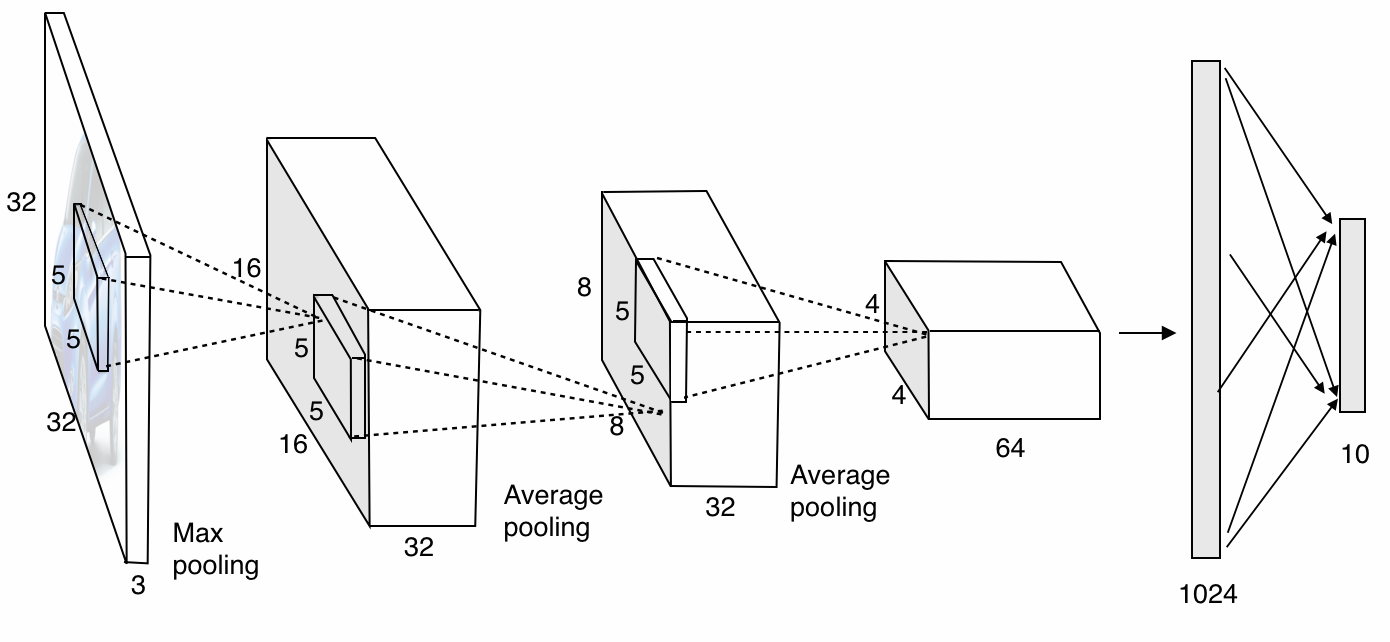
\includegraphics[width=1\textwidth]{architecture}
\caption{The architecture of our CNN.}
\label{fig1}
\end{figure}
\subsection{Sub-model combination}
Let's focus on the penultimate layer in our CNN architecture (Figure~\ref{fig1}). We refer to the already trained CNN model in Figure~\ref{fig1} as the original model. There are totally 1024 units in the penultimate layer, each of which votes for the class membership probabilities $P(Y=i|x,W,b)$, and the importance of each unit's vote is weighted by $W_{ij}$.  The 1024-unit vector of the penultimate layer is denoted as $h_{orig}$.
\par
Now we define a sub-model $m_{i}$ as randomly setting units as zero in the penultimate layer with chance of 50\%, and the remaining units are multiplied by 2:
\begin{equation}
P(h_{m_{i}}^{j}=2h_{orig}^{j})=P(h_{m_{i}}^{j}=0)=\frac{1}{2}.
\end{equation}
where  $h_{m_{i}}$ is the 1024-unit vector of the sub-model $m_{i}$, and $h_{(\cdot)}^{j}$ is the $j$th element of the vector. 
\par
Therefore, the original model can be viewed as a combination of all the possible sub-models:
\begin{equation}
h_{orig} = \lim_{n \to \infty }\frac{1}{n}\sum_{i=1}^{n}h_{m_{i}}=E\left [ h_{m_{i}} \right ]
\end{equation}
For each sub-model, the class membership probability output is denoted as $P_{m_{i}}$. Rather than combining the penultimate layers $h_{m_{i}}$ of the sub-models, we explore the weighted combination of output layer $P_{m_{i}}$ of sub-models:
\begin{equation}
P_{comb} = \sum_{i=1}^{n}l_{i}P_{m_{i}}
\end{equation}
where $l_{i}$ is the weight of each model $m_{i}$, and $P_{comb}$ is the class membership probabilities of the weighted combined model.
\par
Given a set of sub-models $m_{i}, (i = 1,2, ... ,n)$ extracted from the original model $m_{orig}$, the optimal weight $l_{i}$  can be obtained by the following optimization problem:
\par
\setlength{\parindent}{3em}
minimize $\sum_{i=1}^{N}\left \| l^{t}\cdot P_{i}-y_{i} \right \|_{2}^{2}$
\setlength{\parindent}{3em}
subject to $l\succeq 0$

\subsection{Dropout and sub-models}


\section{Multiclass}


\section{Experiments}
\subsection{Sub-model convolutional network}


LDA is a mixture model. It assumes that each document contains various topics, and words in the document are generated from those topics. All documents contain a particular set of topics, but the proportion of each topic in each document is different. 

\par
The generative process of the LDA model can be described as follows:
\par
\setlength{\parindent}{3em}
Given: Dirichlet distribution with parameter vector $\alpha$ of length $K$
\par
Given: Dirichlet distribution with parameter vector $\beta$ of length $V$
\par
for topic number 1 to topic number $K$
\par
\setlength{\parindent}{4em}
draw a word distribution, i.e. a multinomial with parameter vector $\phi _{k}$\par according to $\beta$. $\phi \sim Dirichlet(\beta)$
\par
\setlength{\parindent}{3em}
for document number 1 to topic number $M$
\par
\setlength{\parindent}{4em}
draw a topic distribution, i.e. a multinomial with parameter vector $\theta$ 
\par
according to $\alpha$. $\theta \sim Dirichlet(\alpha)$
\par
for each word in the document
\par
\setlength{\parindent}{5em}
draw a topic $z$ according to $\theta$.  $z \sim Multinomial(\theta)$
\par
draw a word $w$ according to $\phi_{z}$.  $w \sim Multinomial(\phi_{z})$
\setlength{\parindent}{0pt}
\par
Not that $V$ is the cardinality of the vocabulary. The words of a document is observed, but the topic assignment is latent.
\subsection{Training via collapsed Gibbs sampling}
Training data in this project is the words in all documents. The goal of training is to infer the multinomial parameters $\theta$ for each document, and $\phi_{k}$ for each topic.
\par
We use collapsed Gibbs sampling for learning. First it infers the hidden value $z_{nm}$ for each word occurrence in each document: $p(\vec{z}|\vec{w})$. Note $z_{mn}$ is the mixture indicator that chooses the topic for $n$th word in document $m$. $\vec{w}$ is the vector of words making up the entire corpus, and $\vec{z}$ is the corresponding topics.
\par
The idea of Gibbs sampling is assuming that we know the value of $\vec{z}$ for every word occurrence in the corpus except occurrence number $i$, then we draw a $z_{i}$ value for $i$ according to its distribution. Then we assume that this value is known to be true value, and draw a $z_{j}$ for another word, and so on. Eventually this process will converge to a correct distribution $p(\vec{z}|\vec{w})$. Therefore, we need the conditional distribution for a word token with index $i=(m,n)$:
\begin{equation}
p(z_{i}=k|\vec{z}_{-i}, \vec{w}) \propto \frac{n^{(t)}_{k,-i}+\beta}{\sum_{t=1}^{V}(n^{(t)}_{k,-i}+\beta)}(n^{(k)}_{m,-i}+\alpha)
\label{e1}
\end{equation}
where $z_{i}$ is the topic association of $i$th word. $\vec{z}_{-i}$ is $\vec{z}$ with $i$th topic removed. $n^{(t)}_{k}$ is the number of times that word $t$ has been observed with topic $k$. $n^{(k)}_{m}$ refers to the number of times that topic $k$ occurs with a word of document $m$. $n^{(\cdot)}_{\cdot, -1}$ indicates that the word $i$ is excluded from the corresponding document or topic.
\par
Finally, we can obtain the multinomial parameters $\theta$ and $\phi$:
\begin{equation}
\phi_{k,t} = \frac{n^{(t)}_{k}+\beta}{\sum_{t=1}^{V}(n^{(t)}_{k}+\beta)}
\end{equation}
\begin{equation}
\theta_{m,k} = \frac{n^{(k)}_{m}+\alpha}{\sum_{k=1}^{K}(n^{(k)}_{m}+\alpha)}
\end{equation}
where $\phi_{k,t}$ is the multinomial parameter for word $t$ drawn from topic $k$. $\theta_{m,k}$ is the parameter of topic $k$ drawn from document $m$.

\subsection{Goodness-of-fit of the model}
There are two typical ways to evaluate LDA model. 
\subsubsection{Likelihood of held-out data}
\label{section11}
One way is to calculate the probability of held-out documents that are not used for training. The likelihood $p(\vec{w} | \alpha, \beta)$ is intractable, and there are several ways to estimate it.
\par
The probability of the held-out documents $\vec{w}$ given training data $\vec{w'}$ can be written as
\begin{equation}
p(\vec{w}|\vec{w}') = \int \textup{d}\phi \textup{d}\alpha p(\vec{w}| \phi, \alpha)p(\phi, \alpha|\vec{w}')
\end{equation}
 \cite{hanna} approximates this integral by evaluating at a point estimate, and the problem becomes how to evaluate $p(\vec{w}| \phi, \alpha)$. \cite{hanna} summaries several estimating methods: importance sampling methods, harmonic mean method, and annealed importance sampling. \cite{hanna} also proposes two alternative methods: a Chib-style estimator and a ``left-to-right" evaluation algorithm.
\par For example, the frequently used method, Harmonic mean method, estimates the probability as follows
 \begin{equation}
p(\vec{w}| \phi, \alpha) \simeq \frac{1}{\frac{1}{s}\sum _{s}\frac{1}{p(\vec{w}|\vec{z}^{(s)}, \phi)}}
\end{equation}
where $\vec{z}^{(s)}$ is drawn from $p(\vec{z}|\vec{w})$. 
\par
\cite{gabriel} approximates the held-out likelihood with empirical likelihood(EL). It produces a large set of pseudo documents with parameter $\alpha$ and $\beta$, and the pseudo documents are then used to train a tractable model.
 The true likelihood of the test set is then estimated as its likelihood under the tractable model. 
 \par
 Perplexity is another way to calculate the likelihood. It is defined as the reciprocal geometric mean of the token likelihoods in the test corpus given the model:
 \begin{equation}
 p(\vec{W}|M)=\textup{exp}-\frac{\sum_{m=1}^{M}\textup{log}p(\tilde{\vec{w}}_{\tilde{m}}|M)}{\sum_{m=1}^{M}N_{m}}
 \end{equation}
where $M$ is the trained model, and $\vec{w}_{\tilde{m}}$ is the word vector in document $\tilde{m}$. Lower values of perplexity indicate lower misrepresentation of the words of the test documents by the trained topics.
 \par
 The log-likelihood can be expressed as:
 \begin{equation}
 \textup{log}p(\tilde{\vec{w}}_{\tilde{m}}|M) = \sum_{t=1}^{V}n^{(t)}_{\tilde{m}}\textup{log}(\sum_{k=1}^{K}\phi_{k,l}\cdot\theta_{\tilde{m},k})
 \end{equation}
 where $n^{(t)}_{\tilde{m}}$ is the number of times word $t$ occurs in document $\tilde{m}$.
 
\subsubsection{Evaluation of clustering result}
Another way to evaluate the model is to measure its performance on some secondary tasks, for example, document classification or clustering. The LDA model provides a soft clustering of the documents. The evaluation of clustering quality can be done in many ways: 
\begin{enumerate}
  \item  We can simply check if the most frequent words generated from each topic are semantically related.
  \item  We can also check if intra-class document similarity is higher than inter-class document similarity.
  \item  When we have the label of each document, and the number of topics $K$ equals the number of given labels, we can convert the soft clustering result into a hard result, and calculate the categorization accuracy. Converting soft clustering to a hard one is simply done by assigning topic with highest probability to each document. 
  \item We can also directly compare the soft clustering result with the priori categorization(\cite{gregor}). Variation of Information distance (VI-distance) can be used to compare the two clusterings. It assumes two distributions over class for each document: $p(c=j|d_{m})$ and $p(z = k|d_{m})$, where $j\in [1,J]$  and $k\in [1,K]$ are the class labels or topics of the two distribution. Note that $K$ doesn't need to be the same with $J$. $d_{m}$ is $m$th document. The class probabilities are obtained by averaging over the corpus:$p(c=j)=\frac{1}{M}\sum _{m}p(c=j|d_{m})$ and $p(z=k)=\frac{1}{M}\sum _{m}p(z=k|d_{m})$. The joint probability of co-occurring pairs is $p(c=j, z = k)=\frac{1}{M}\sum _{m}p(c=j|d_{m})p(z=k|d_{m})$. Then the VI-distance measure is defined as follow:
  \begin{equation}
D_{VI}(C,Z)=H(C)+H(Z)-2I(C,Z)
\end{equation}
with
  \begin{equation}
I(C,Z) = \sum_{j=1}^{J} \sum_{k=1}^{K}p(c=j,z=k)[\textup{log}_{2}p(c=j,z=k)-\textup{log}_{2}p(c=j)p(z=k)]
  \end{equation}
  \begin{equation}
H(C)=-\sum_{j=1}^{J} p(c=j)\textup{log}_{2}p(c=j)
    \end{equation}
  \begin{equation}
H(Z)=-\sum_{k=1}^{K} p(z=k)\textup{log}_{2}p(z=k)
    \end{equation}
    VI-distance is always nonnegative, and smaller VI-distance indicates the two clustering are more similar.
\end{enumerate}
\subsection{Overfitting monitoring}
In Section~\ref{section11}, we introduce several ways to calculate the likelihood of held-out data. In addition to using likelihood or perplexity to evaluate the goodness-of-fit, we can also use it to monitor overfitting. By calculating likelihood/perplexity of the training data, and comparing it with likelihood/perplexity of test data, we can get the idea whether overfitting occurs. When no overfitting occurs, the difference between two types of likelihood should remain low.


\section{Implementation of algorithm}
Algorithms are realized in Python.
%\subsection{Implementation of training algorithm}
\paragraph{Data} \hspace{0pt} The vocabulary of words is very large. However, in one document, only a small part of the vocabulary occurs, and there is no need to traverse every word in vocabulary for each document. Therefore, word counts of all documents are stored in \texttt{scipy.sparse.csc\_matrix}, a compressed sparse column matrix. Non-zero values can be efficiently located, so the training process can be speeded up.
\paragraph{Initialization} \hspace{0pt} The hyperparameters $\alpha$, $\beta$, and $K$ are predefined. The initial topics $z_{mn}$ associating with words $w_{mn}$ are random number ranging from $1$ to $K$. For words in all documents, the counts $n^{(t)}_{k}$ and $n^{(k)}_{m}$ are calculated. 
\paragraph{Gibbs sampling} \hspace{0pt} The counts $n^{(t)}_{k}$ and $n^{(k)}_{m}$ are stored in matrices. Instead of looping over $K$ to calculate the conditional probability $p(z_{i}=k|\vec{z}_{-i}, \vec{w})$ for each topic $k$, we use matrix operation to calculate unnormalized conditional probability of all topics. This is faster than simply looping over $K$ topics for each word.
\paragraph{Visualization of clustering result} \hspace{0pt} To evaluate the clustering result in an intuitive manner, we draw a mapping from a document to a 3D point according to each document's multinomial parameter $\theta$. When there are 3 topics or less, we can simply assign each topic to one axis. In this way, each coordinate corresponds to one topic distribution ($\theta$). When there are more than 3 topics, we use principle component analysis (PCA) to reduce the dimension. Three principle components are extracted, and then each documents can be mapped to a 3D point. We use points with different colors and shapes to represent different classes of documents. Therefore we can observe classification result as well as clustering result in the 3D image.
\label{implementation}
%\subsection{Implementation of training algorithm}


\section{Design of experiments}
\subsection{Datasets}
We use two datasets for experiments. The first is Classic400 dataset \footnote{ http://cseweb.ucsd.edu/users/elkan/151/classic400.mat}. It consists of 400 documents, with a vocabulary of 6205 words. There are 3 categories of the documents. The second dataset we use is the BBC Sports dataset \footnote{http://mlg.ucd.ie/datasets/bbc.html}. It consists of 737 documents with a vocabulary of 4613 words. There are 5 classes of the documents. For both datasets, we randomly choose10\% from each category as test data, and 90\% as training data.

\subsection{Choice of hyperparameters}
We use perplexity and VI-distance as the criteria to choose the three hyperparameters: $\alpha$, $\beta$, and $K$. 
Best choices of $\alpha$ and $K$ have strong correlation, as is shown in \cite{finding},  which chooses hyperparameters as $\alpha = 50/K$, $\beta=0.1$. For both datasets, we have the true label of every document. Therefore, an intuitive guess of $K$ would be the number of classes. Grid search for all three hyperparameters requires too much work, so we first fix $K$ as the number of classes, and apply grid search of $\alpha$ and $\beta$. After deciding best $\alpha$ and $\beta$ for fixed $K$, we then search for best $K$ with fixed $\beta$ and changing $\alpha$, under the assumption that $\alpha \propto \frac{1}{K}$.
\subsection{Evaluating results}
We use several ways to evaluate the models:
\begin{enumerate}
  \item We look at the 10 highest-probability words for each topic, to see if topics we learn are meaningful.
  \item  We calculate perplexity of training data and perplexity of test data for every 5 epochs, to check convergence and check overfitting.
  \item We calculate VI-distance of training data to monitor clustering result.
  \item We visualize the clustering result in 3 dimensional space.
  \item We also compare the running time of each Gibbs sampling epoch of the two models.
\end{enumerate}

\section{Experimental results}
\subsection{Classic400 dataset}
\subsubsection{Best hyperparameters}
By fixing $K$ at 3, we use grid search for pairs ($\alpha, \beta$). We choose from $\alpha = \left\{0.01, 0.1, 1\right\} = \left\{0.03/K, 0.3/K, 3/K\right\}$, and $\beta =\left\{0.1, 1, 2\right\}$. Figure~\ref{1} shows the visualizing result of the 9 pairs of parameters, and Table~\ref{table1} shows the corresponding perplexity and VI-distance.
\par
From Figure~\ref{1}, we can see the role of $\alpha$. For smaller $\alpha$, documents in each cluster are more scattered; for larger $\alpha$, different clusters are more separated, and the documents are prone to locate in three corners of the triangle. This is also illustrated in Table~\ref{table1}, where VI-distance increases with $\alpha$. This observation is intuitive: $\alpha$ is the pseudo count of topic per document. Larger $\alpha$ will bring an averaging effect of different topics.
\par
From Table~\ref{table1}, we can observe the role of $\beta$. For smaller $\beta$, perplexity of training data is smaller. However, perplexity of test data doesn't change much with $\beta$. $\beta$ is the pseudo count of word per document. Larger $\beta$ brings a larger averaging effect of all the words, therefore making the model not so fit for training data. 
\par
We choose $(\alpha =0.3/K, \beta = 1)$ as the best parameter pairs, to achieve low perplexity and VI-distance.
\par
\begin{figure}
\centering 
\subfigure[$\alpha = 0.01$, $\beta = 0.1$]{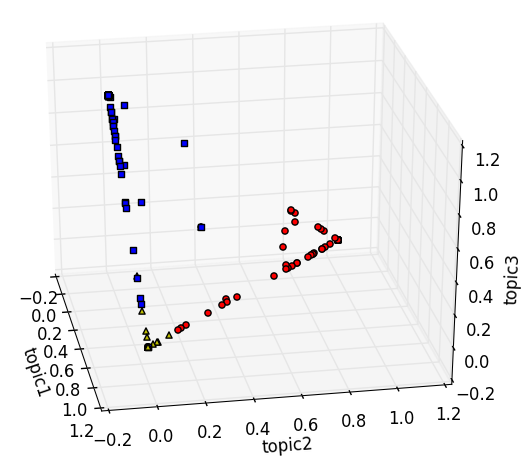
\includegraphics[width=0.3\textwidth]{1.png}} 
\subfigure[$\alpha = 0.01$, $\beta = 1$]{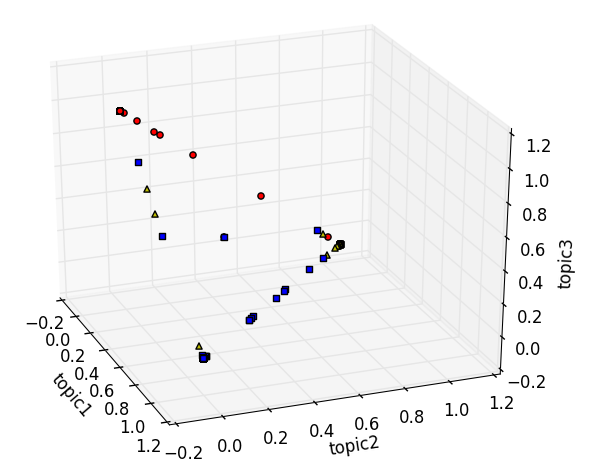
\includegraphics[width=0.3\textwidth]{2.png}} 
\subfigure[$\alpha = 0.01$, $\beta = 2$]{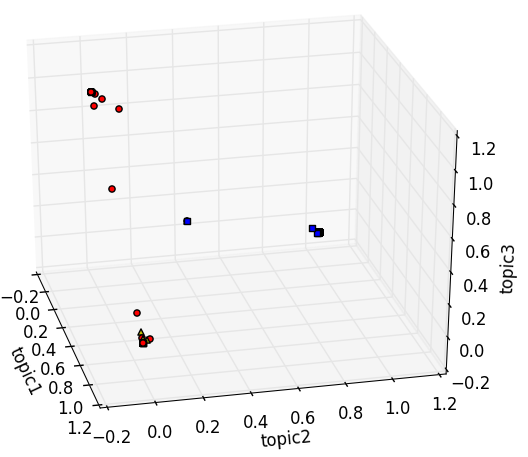
\includegraphics[width=0.3\textwidth]{3.png}} 
\subfigure[$\alpha = 0.1$, $\beta = 0.1$]{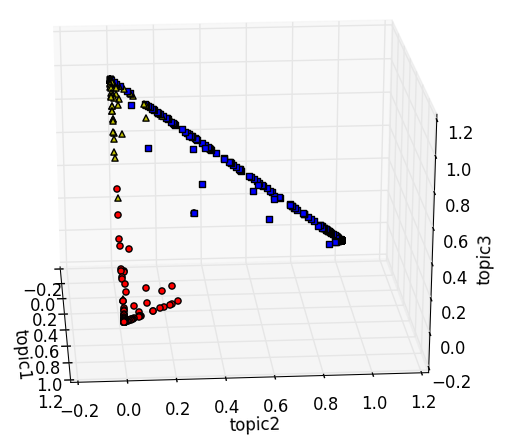
\includegraphics[width=0.3\textwidth]{4.png}} 
\subfigure[$\alpha = 0.1$, $\beta = 1$]{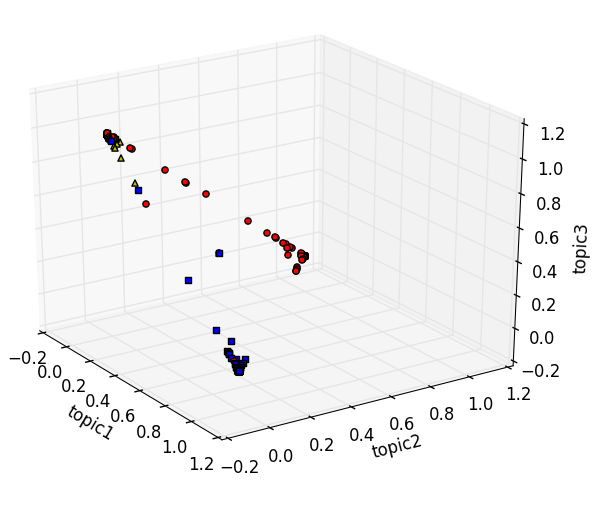
\includegraphics[width=0.3\textwidth]{5.png}} 
\subfigure[$\alpha = 0.1$, $\beta = 2$]{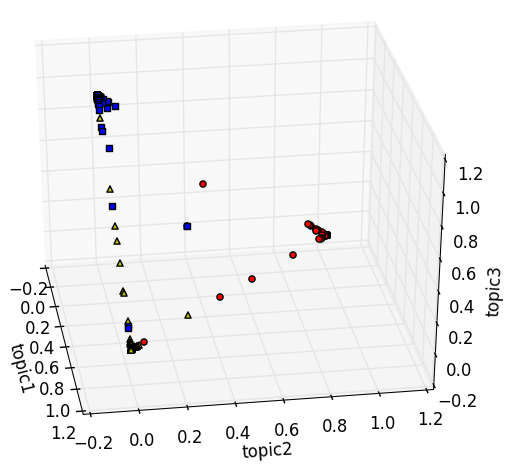
\includegraphics[width=0.3\textwidth]{6.png}} 
\subfigure[$\alpha = 1$, $\beta = 0.1$]{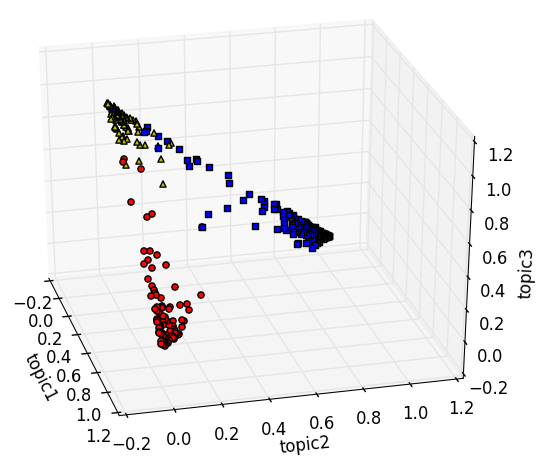
\includegraphics[width=0.3\textwidth]{7.png}} 
\subfigure[$\alpha = 1$, $\beta = 1$]{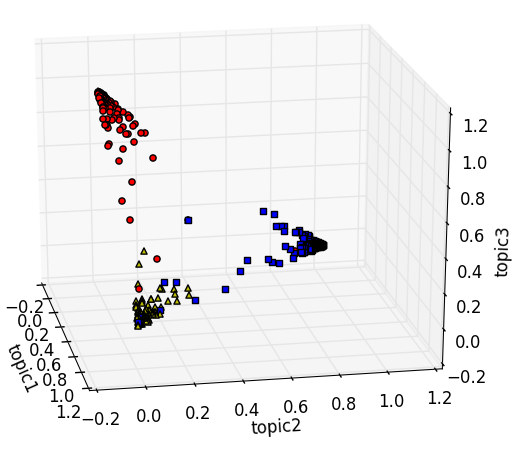
\includegraphics[width=0.3\textwidth]{8.png}} 
\subfigure[$\alpha = 1$, $\beta = 2$]{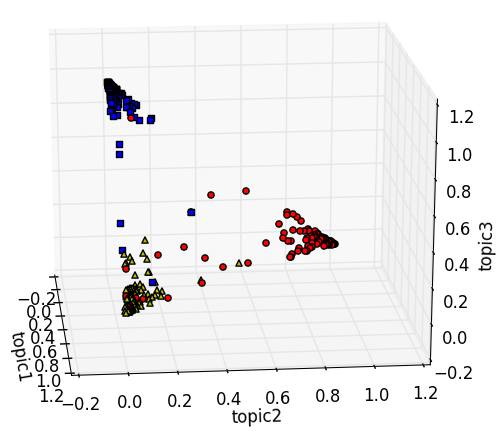
\includegraphics[width=0.3\textwidth]{9.png}} 
\caption{ Plots of Classic400 dataset with $K= 3$ and varying $\alpha$ and $\beta$.} \label{1} 
\end{figure}
\begin{table}
\centering 
    \begin{tabular}{|l|l|l|l|}
    \hline
    Parameter($\alpha, \beta$)  & Perplexity (training) & Perplexity (test)  & VI-distance (training)  \\ \hline
    (0.01, 0.1)   & 1376.024120           & 2500.267304                                     & 0.796688               \\ \hline
    (0.01,1)      & 1803.455444           & 2303.252994                                     & 1.381389               \\ \hline
    (0.01,2)      & 2088.023795           & 2506.341132                                     & 0.909851               \\ \hline
    (0.1,0.1)     & 1451.690149           & 2646.197142                                     & 1.387363               \\ \hline
    (0.1,1)       & 1753.193891           & 2256.134722                                       & 0.801898               \\ \hline
    (0.1,2)       & 2071.336636           & 2462.702027                                       & 0.704664               \\ \hline
    (1,0.1)       & 1484.825815           & 2536.642742                                       & 1.567750               \\ \hline
    (1,1)         & 1802.399166           & 2310.176229                                       & 1.260563               \\ \hline
    (1,2)         & 2128.084925           & 2492.720476                                       & 1.362268               \\ \hline   
    \end{tabular}
     \caption{Perplexity and VI-distance of Classic400 dataset, with $K= 3$ and varying $\alpha$, $\beta$.}   
     \label{table1}
\end{table}
Then, we fix $\beta = 1$, $\alpha = 0.3/K$, and search for best K. We check perplexity, VI-distance and the mapping image for $K = \left\{2,3,4,5\right\}$. Figure~\ref{2} shows visualization of clustering results with different $K$. For different $K$, location of points forms different 3D shapes: for $K = (2,3,4,5)$, the shapes are line, triangle, tetrahedron, tetrahedron with an extra point in the middle, respectively. Points reside in vertex of those shapes. Table~\ref{table2} shows the evaluation of goodness-of-fit. $K=3$ achieves best perplexity on test data and VI-distance. Training perplexity decreases with larger $K$, because when we have larger topic number we have more parameters to fit the training data, however, bigger $K$ causes overfitting: Test perplexity increases when $K$ is big, this is because when $K$ becomes too large, the number of parameters are too large for the training data. Therefore, we choose $K = 3$ as the best parameter.
\begin{figure}
\centering 
\subfigure[$K=2$, $\alpha = 0.15$]{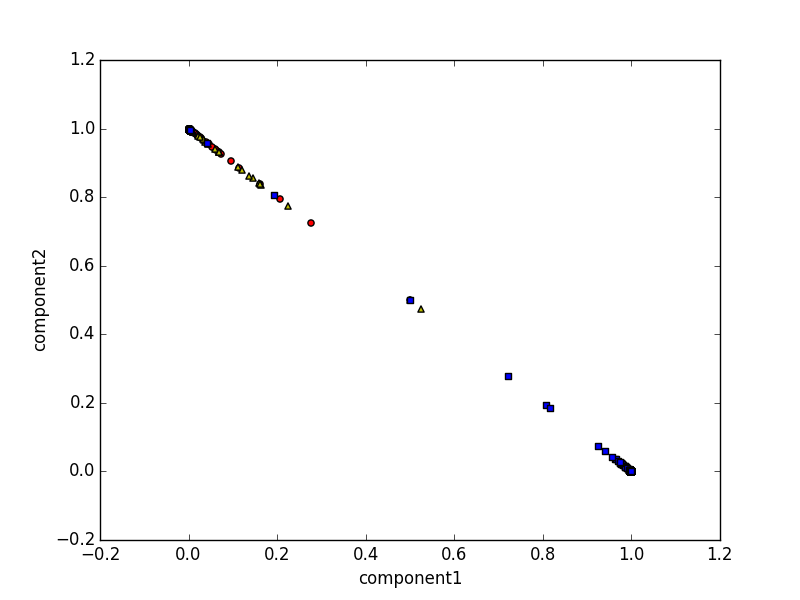
\includegraphics[width=0.4\textwidth]{12.png}} 
\subfigure[$K=3$, $\alpha = 0.1$]{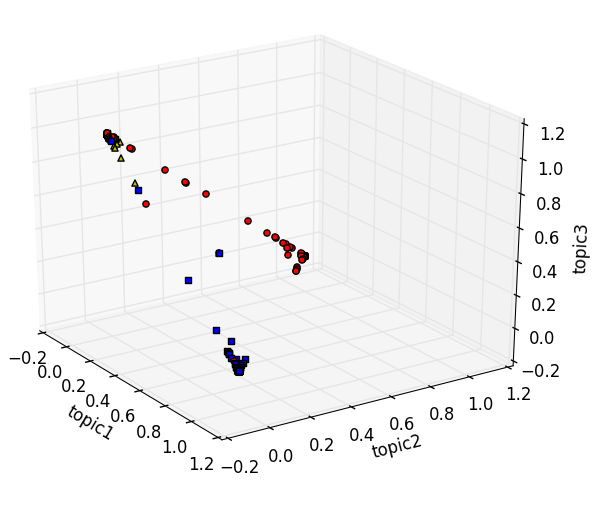
\includegraphics[width=0.4\textwidth]{5.png}} 
\subfigure[$K=4$, $\alpha = 0.075$]{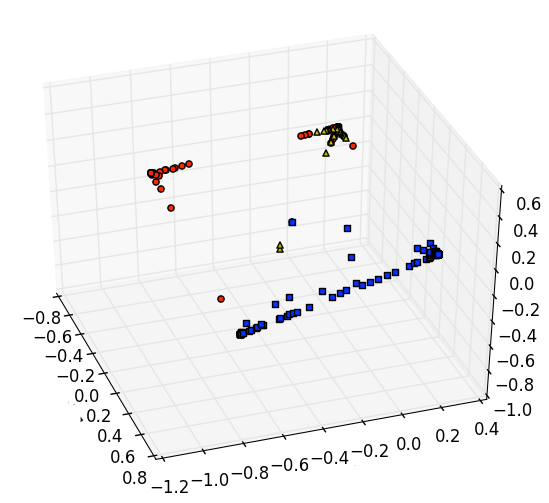
\includegraphics[width=0.4\textwidth]{10.png}} 
\subfigure[$K=5$, $\alpha =0.06 $]{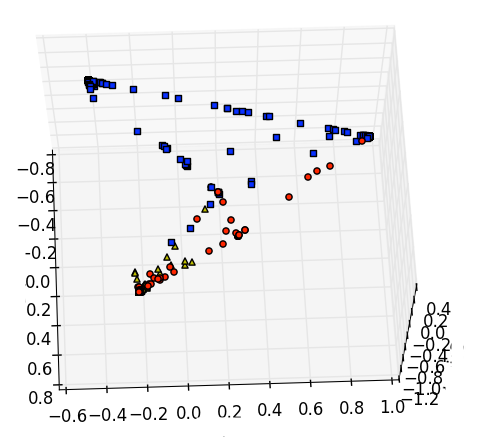
\includegraphics[width=0.4\textwidth]{11.png}} 
\caption{ Plots of Classic400 dataset with $\beta= 1, \alpha = 0.3/K$ and varying $K$.} \label{2} 
\end{figure}

\begin{table}
\centering
    \begin{tabular}{|l|l|l|l|}
    \hline
    Parameter(K) & Perplexity (training) & Perplexity (test) & VI-distance(training) \\ \hline
    2            & 1931.919028                     & 2415.384221                 & 0.864250                     \\ \hline
    3            & 1753.193891           & 2256.134722       & 0.801898              \\ \hline
    4            & 1718.810470           & 2283.469816       & 1.339418              \\ \hline
    5            & 1704.840676           & 2364.641784       & 1.864304              \\ \hline
    \end{tabular}
    \caption{Perplexity and VI-distance of Classic400 dataset, with $\beta= 1,  \alpha = 0.3/K$ and varying $K$}
\label{table2}
\end{table}
\subsubsection{Evaluation results}
We have decided the parameters to be $K = 3, \alpha = 0.3/K, \beta =1$. Then, we evaluate the model.
\par
Figure~\ref{per1} shows training and test perplexity of the model with number of epochs. Perplexity on test data is higher than that on training data, and the dropping rate of test perplexity is slightly lower. However, the trend of the two perplexities are similar. Therefore, we could infer there may exist slight overfitting, this may be caused by lack of data (we only have 360 training documents). According to the figure, the model converges after 60 epochs.
\par
Table~\ref{table3} shows 10 words that most frequently occur in each topic. In each topic, words are semantically related, and they are related to the true topic assigned by human. This means the model we train has a good clustering for the topics, with semantic meaning.
\par
We calculate the average running time for every epoch of Gibbs sampling. The average running time of one epoch is 3.3649 seconds, which is shown in Table~\ref{table7}. 
\begin{figure}
\centering
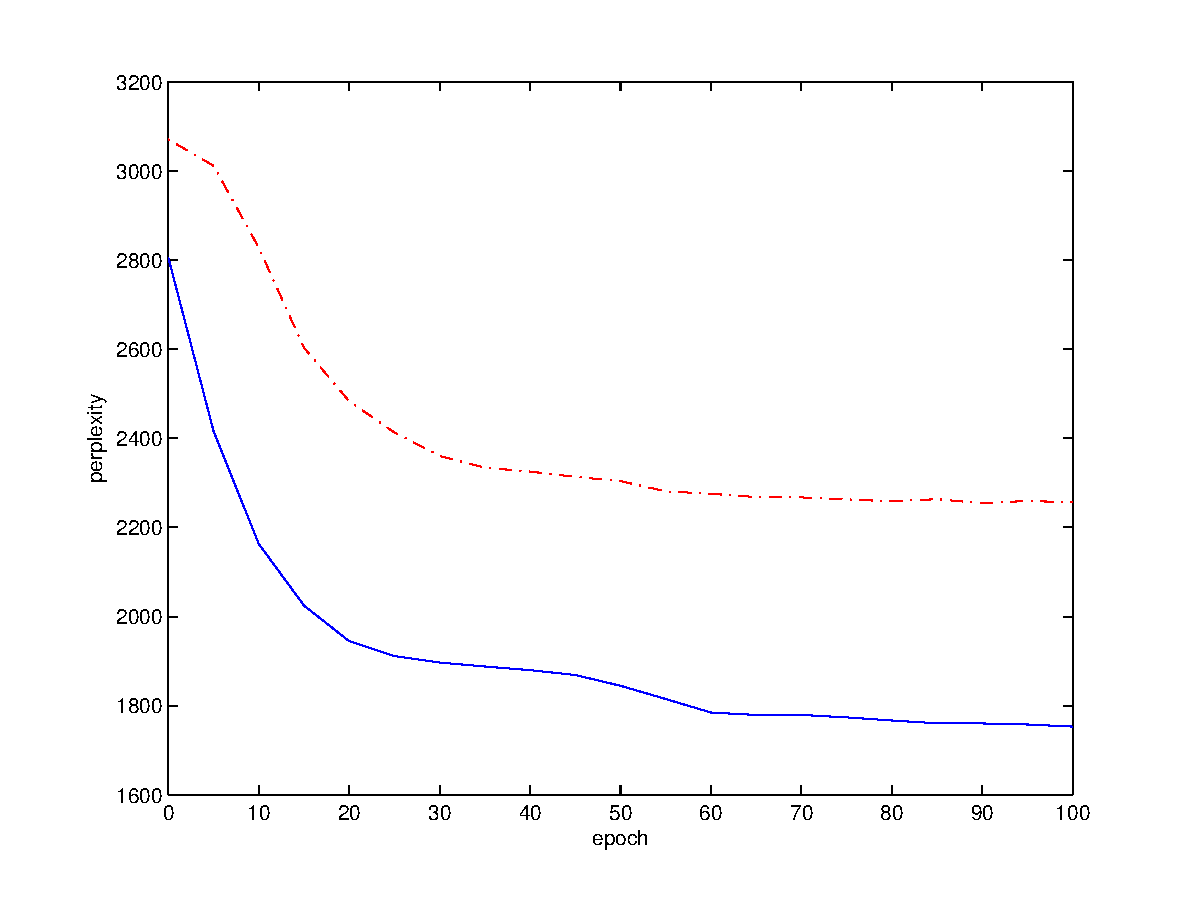
\includegraphics[width=0.8\textwidth]{perplex1}
\caption{Training and test perplexity of LDA model for Classic400. Blue hard line: training data; Red dash-dot line: test data.}
\label{per1}
\end{figure}
\begin{table}
\centering
    \begin{tabular}{|l|l|}
    \hline
    Topic                      & Ten most frequent words                                                            \\ \hline
    1: 'Medical'           & patients  fatty  acids  nickel  ventricular  aortic  cases  left  glucose  septal   \\ \hline
    2:'Scientific methods' & system  scientific  retrieval  research  language  science  methods                 \\
    ~                          &  systems  subject  journals                                                         \\ \hline
    3:'aero-physics'       & boundary  layer  wing  supersonic  velocity  mach  wings  ratio  jet  plate         \\ \hline
    \end{tabular}
    \caption{Top 10 frequent words for each topic of LDA model for Classic400.}
    \label{table3}
    \end{table}
\subsection{BBCSport dataset}
\subsubsection{Best hyperparameters}
First we fix $K=5$, which is the number of labels given. With the experience in Classic400 dataset, this time we do the grid search for $\alpha = \left\{0.3/K, 3/K\right\}, \beta = \left\{1, 2\right\}$. Figure~\ref{4} shows the visualization result of four models with each parameter pair. Table~\ref{table4} shows the perplexity and VI-distance of the corresponding models. 
\par
From Figure~\ref{4}, we can see that when $\alpha$ increases, the documents are more scattered. Note that there are 5 topics, and PCA cannot separate them entirely on the 3D image. From Table~\ref{table4}, we observe that larger $\beta$ leads to larger perplexity on both training and test data. VI-distance is larger with larger $\alpha$. These trends are similar with what we observe at Classic400 dataset. For best perplexity and VI-distance, we choose the pair $(\alpha=0.3/K, \beta=1)$.
\begin{figure}
\centering 
\subfigure[$\alpha=0.06$, $\beta = 1$]{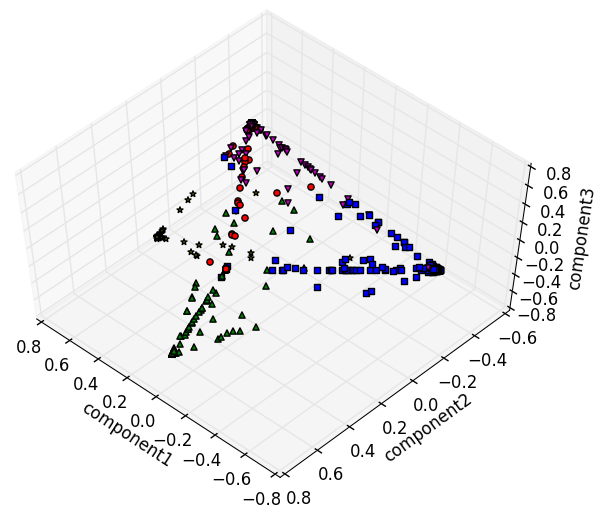
\includegraphics[width=0.4\textwidth]{13.png}} 
\subfigure[$\alpha=0.06$, $\beta = 2$]{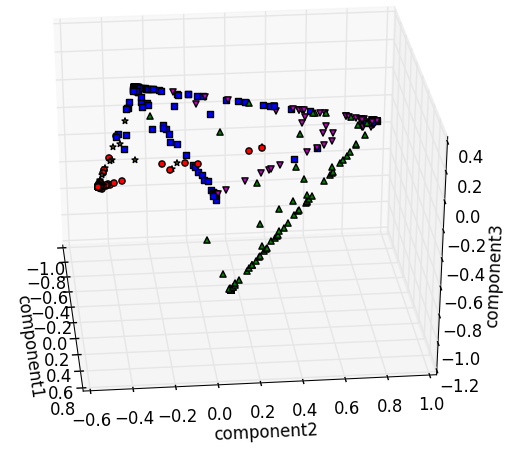
\includegraphics[width=0.4\textwidth]{14.png}} 
\subfigure[$\alpha=0.6$, $\beta = 1$]{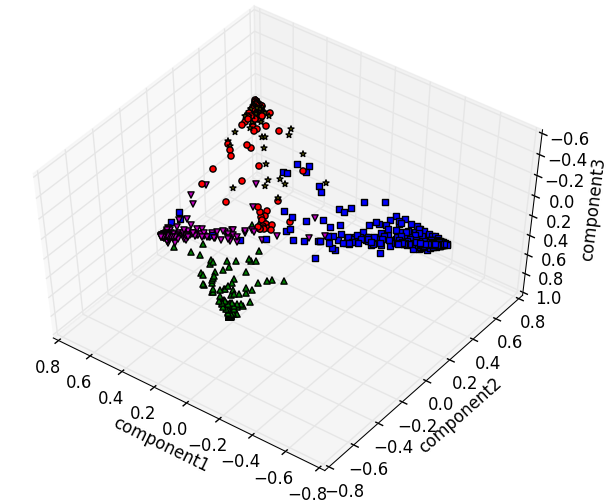
\includegraphics[width=0.4\textwidth]{15.png}} 
\subfigure[$\alpha=0.6$, $\beta = 2$]{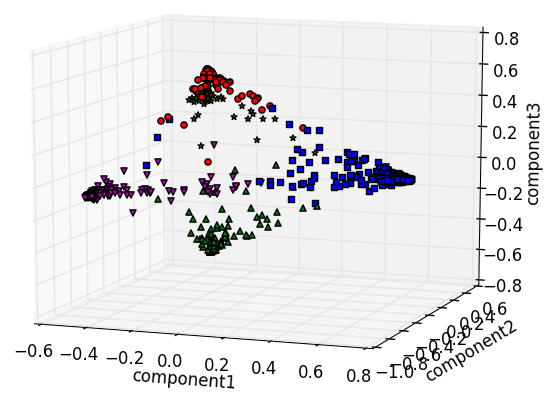
\includegraphics[width=0.4\textwidth]{16.png}} 
\caption{ Plots of BBCSports dataset with $K= 5$ and varying $\beta$ and $\alpha$.} 
\label{4} 
\end{figure}
\begin{table}
\centering 
    \begin{tabular}{|l|l|l|l|}
    \hline
    Parameters ($\alpha, \beta$) & Perplexity(training) & Perplexity(test) & VI-distance \\ \hline
    (0.06,1)      & 1194.730739          & 1413.515161      & 1.836619    \\ \hline
    (0.06,2)      & 1278.352876          & 1499.750074      & 1.735083    \\ \hline
    (0.6,1)       & 1207.601372          & 1434.633843      & 2.127757    \\ \hline
    (0.6,2)       & 1282.181586          & 1491.711059      & 2.013811    \\ \hline
    \end{tabular}  
    \caption{Perplexity and VI-distance of BBCSport dataset, with $K= 5$ and varying $\alpha$, $\beta$.}   
     \label{table4}
\end{table}
Then, we fix $(\alpha=0.3/K, \beta=1)$ and change $K$, with $K = \left\{3,4,5,6\right\}$. From Figure~\ref{5} and Table~\ref{5}, we choose $K=5$, with lowest perplexity in both training and test data, and low VI-distance.
\par
Therefore, the hyperparameters we choose are $K = 5, \alpha = 0.3/K, \beta = 1$.
\begin{table}
\centering
    \begin{tabular}{|l|l|l|l|}
    \hline
    Parameter (K) & Perplexity(training) & Perplexity(test) & VI-distance \\ \hline
    3             & 1347.412626          & 1610.204673      & 1.691689    \\ \hline
    4             & 1272.958416          & 1498.080381      & 1.801365    \\ \hline
    5             & 1163.215412          & 1395.538324      & 1.671155    \\ \hline
    6             & 1155.549721          & 1402.170199      & 2.183145    \\ \hline
    \end{tabular}
    \caption{Perplexity and VI-distance of BBCSport dataset, with $\beta= 1, \alpha = 0.3/K$ and varying $K$}
\label{table5}
\end{table}
\begin{figure}
\centering 
\subfigure[$K=3$, $\alpha = 0.1$]{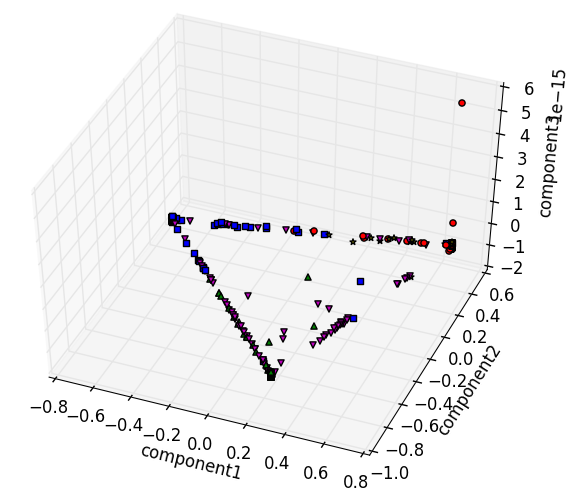
\includegraphics[width=0.4\textwidth]{bbc3.png}} 
\subfigure[$K=4$, $\alpha = 0.075$]{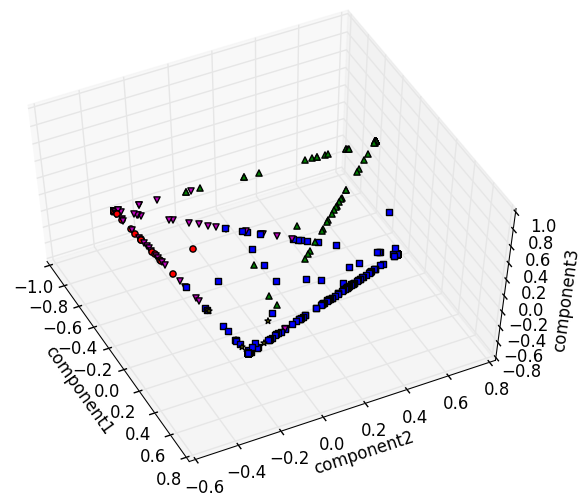
\includegraphics[width=0.4\textwidth]{bbc4.png}} 
\subfigure[$K=5$, $\alpha = 0.06$]{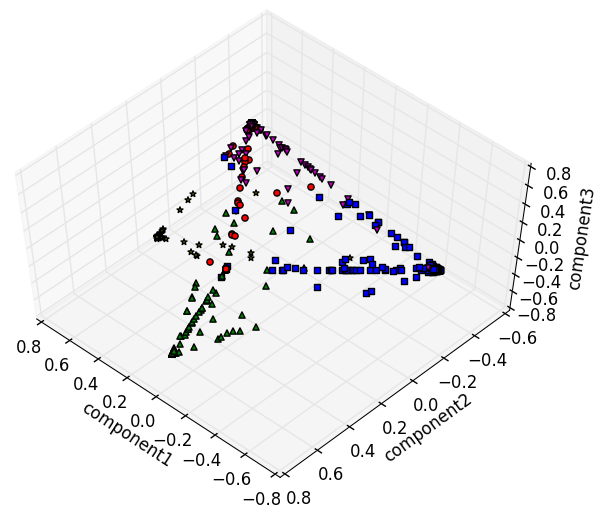
\includegraphics[width=0.4\textwidth]{13.png}} 
\subfigure[$K=6$, $\alpha =0.05 $]{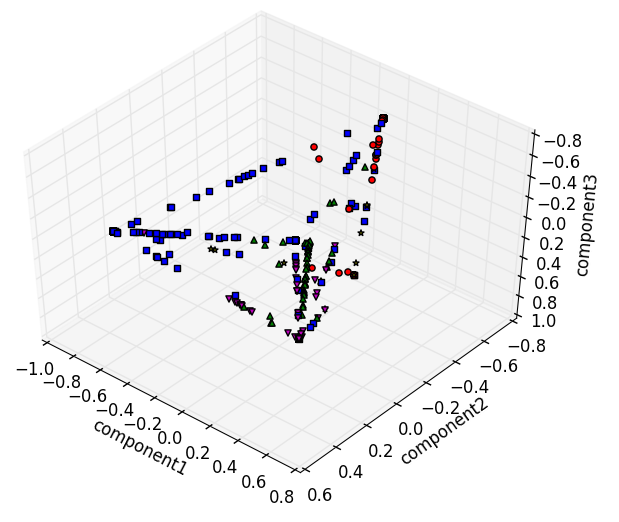
\includegraphics[width=0.4\textwidth]{bbc6.png}} 
\caption{ Plots of BBCSport dataset with $\beta= 1, \alpha = 0.3/K$ and varying $K$.} 
\label{5} 
\end{figure}

\subsubsection{Evaluation results}
\begin{table}
\centering
    \begin{tabular}{|l|l|}
    \hline
    Topic        & Ten most frequent words                                                   \\ \hline
    1: Rugby     & england  wale  game  ireland  rugbi  against  nation  plai  six  player   \\ \hline
    2: Athletics & olymp  world  athlet  race  year  indoor  athen  test  champion  win      \\ \hline
    3: Cricket   & test  cricket  plai  england  first  seri  south  match  run  australia   \\ \hline
    4:  Football & game  player  club  plai  chelsea  arsen  unit  leagu  goal  footbal      \\ \hline
    5: Tennis    & plai  open  win  match  first  set  year  final  game  roddick            \\ \hline
    \end{tabular}
    \caption{Top 10 frequent words for each topic of LDA model for BBCSport.}
    \label{table6}
\end{table}
\begin{figure}
\centering
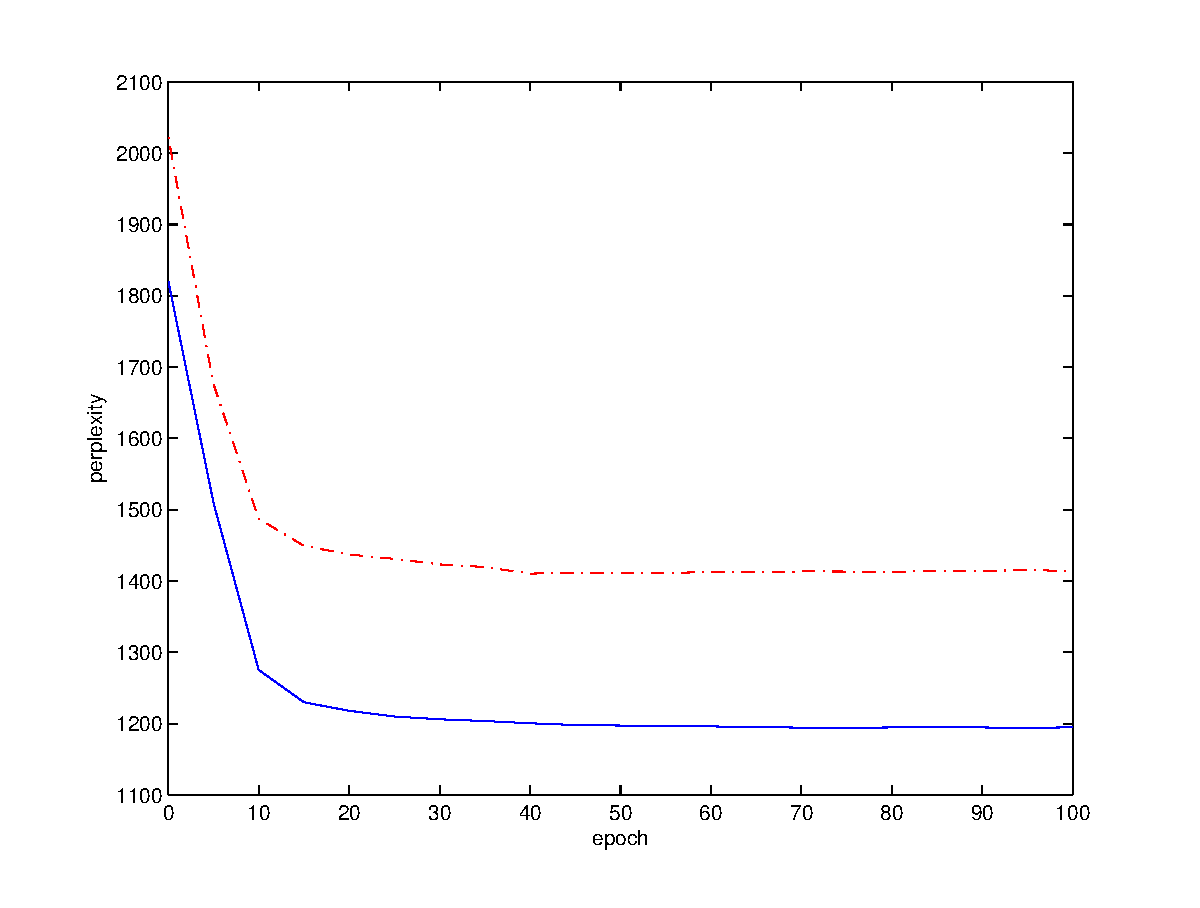
\includegraphics[width=0.8\textwidth]{perplex2}
\caption{Training and test perplexity of LDA model for BBCSport. Blue hard line: training data; Red dash-dot line: test data.}
\label{per2}
\end{figure}
Figure~\ref{per2} shows training and test perplexity of the model as number of epochs increases. Perplexity on test data is still higher than that on training data, and the dropping rate of test perplexity is slightly lower. Compared with Figure~\ref{per2}, we can see that model of BBCSport has less overfitting than Classic400's model. The reason may be there being more training data in this BBCSport dataset: BBCSport training set has 109579 words in total, while Classic400 training set has only 27415 words. Although BBCSport dataset needs to train more parameters, it still has larger dataset-parameter ratio. From the figure, we can also observe rate of convergence of the model. The model converges after 40 epochs.
\par
Table~\ref{table6} shows ten words that most frequently occur in each topic. The words in the dataset are pre-processed before training: Stemming is performed. This avoids a word of different tense or a word in plural form being regarded as a different word. Since we only care about the topic related to the words, eliminating the impact of tense or plural form is sensible. Note that $K=5$ is the true label number, therefore we can assign each topic to a label, judging by the semantic meaning of the top 10 words. Some words are very closely related to the label, for example, ``chelsea", ``arsen" (which stands for arsenal) are strongly related to football. There are other words that are shared by some topics, for example, ``year", ``win" and ``plai" are shared by two or three topics. This is because the five topics are all about sports. They are semantically close to each other, and share some words that associate with all kinds of sports.
\par
From one training process, we calculate the average running time for every epoch of Gibbs sampling. The average running time of one epoch is 12.3923 seconds, as is shown in Table~\ref{table7}. The normal time to perform one epoch of Gibbs sampling is $O(NK)$, where $N$ is the total number of words in all documents. However, as is described in Section~\ref{implementation}, we can make the time much less relevant to $K$ by using matrix operation, making the time comparable to $O(N)$ when $K$ is not too large. This is also illustrated in Table~\ref{table7}: For BBCDataset, increasing $K$ from 5 to 20 doesn't affect running time much. When $K$ becomes 1000, there is a noticeable time increase. Therefore, one-epoch running time for BBCSport dataset is approximately 4 times of Classic400 dataset, which is proportional to their word number ratio. 
\begin{table}
\centering
    \begin{tabular}{|l|l|l|l|}
    \hline
    Datasets   & Number of topics: K & Total number of words:N & Running time (s) \\ \hline
    Classic400 & 3                   & 27415                   & 3.3649           \\ \hline
    BBCSport   & 5                   & 109579                  & 12.3923          \\ \hline
    BBCSport   & 6                   & 109579                  & 12.3834          \\ \hline
    BBCSport   & 10                  & 109579                  & 12.1788          \\ \hline
    BBCSport   & 20                  & 109579                  & 11.9438                \\ \hline
    BBCSport   & 1000                 & 109579                  & 18.0922          \\ \hline
    \end{tabular}
    \caption{Comparison of running time of two datasets.}
    \label{table7}
\end{table}

\section{Conclusions}
%In this project, we realize a fast implementation of CRFs and test it on the provided dataset. We train the model by three different methods. From the experiment result, we find that contrastive divergence is slightly better than stochastic gradient ascent because it is faster and can achieve equivalent performance on the test set. The model trained by Collins perceptron is the worst for its ``carelessness". Feature design is crucial for the system performance. Human-engineered feature functions can make great improvement since they are more discriminative. Duplicating can help improve class-specific accuracy. Also, overflow can be effectively solved by the logsumexp trick.

In this project, we realize the LDA model by Gibbs sampling, and evaluate it on two datasets. We use multiple types of evaluation criteria to check performance of the model. From the experiment results, we find that hyperparameters have different roles in the model: increasing $\alpha$ makes document clusters more scattered; smaller $\beta$ results in smaller perplexity when no overfitting occurs; and larger topic number $K$ makes training perplexity smaller but may cause overfitting. The perplexity results of two datasets suggest probable overfitting, which is caused by insufficient data. However, we can observe that latter dataset with larger data gets less overfitting. One problem of this implementation of LDA model is that it is not well scalable. Training time for one epoch is proportional to scale of dataset. Therefore training will become very slow with a large dataset.

\bibliographystyle{splncs}
\bibliography{ECE273}
\end{document}